% Opcje klasy 'iithesis' opisane sa w komentarzach w pliku klasy. Za ich pomoca
% ustawia sie przede wszystkim jezyk i rodzaj (lic/inz/mgr) pracy, oraz czy na
% drugiej stronie pracy ma byc skladany wzor oswiadczenia o autorskim wykonaniu.
\documentclass[declaration,shortabstract,mgr,masc,english]{iithesis}

\usepackage[utf8]{inputenc}

%%%%% DANE DO STRONY TYTUŁOWEJ
% Niezaleznie od jezyka pracy wybranego w opcjach klasy, tytul i streszczenie
% pracy nalezy podac zarowno w jezyku polskim, jak i angielskim.
% Pamietaj o madrym (zgodnym z logicznym rozbiorem zdania oraz estetyka) recznym
% zlamaniu wierszy w temacie pracy, zwlaszcza tego w jezyku pracy. Uzyj do tego
% polecenia \fmlinebreak.
\polishtitle    {Parsing zależnościowy za pomocą sieci neuronowej}
\englishtitle   {End-to-End neural dependency parsing}
\polishabstract {\ldots}
\englishabstract{\ldots}
% w pracach wielu autorow nazwiska mozna oddzielic poleceniem \and
\author         {Michał Zapotoczny}
% w przypadku kilku promotorow, lub koniecznosci podania ich afiliacji, linie
% w ponizszym poleceniu mozna zlamac poleceniem \fmlinebreak
\advisor        {dr Jan Chorowski}
%\date          {}                     % Data zlozenia pracy
% Dane do oswiadczenia o autorskim wykonaniu
\transcriptnum {248100}                     % Numer indeksu
\advisorgen    {dr. Jana Chorowskiego} % Nazwisko promotora w dopelniaczu
%%%%%

%%%%% WLASNE DODATKOWE PAKIETY
%
% \usepackage{import,graphicx,listings,amsmath,amssymb,amsthm,amsfonts,tikz}
\usepackage{graphicx,float,import,microtype}%,import,color,microtype}
\usepackage{amsmath,amsthm,float}
\let\lll\undefined
\usepackage{amssymb} % http://www.rexamine.com/2013/04/latex-polish-babel-and-amssymb-conflict/
\usepackage{wrapfig}


%
%%%%% WŁASNE DEFINICJE I POLECENIA
%
%\theoremstyle{definition} \newtheorem{definition}{Definition}[chapter]
%\theoremstyle{remark} \newtheorem{remark}[definition]{Observation}
%\theoremstyle{plain} \newtheorem{theorem}[definition]{Theorem}
%\theoremstyle{plain} \newtheorem{lemma}[definition]{Lemma}
%\renewcommand \qedsymbol {\ensuremath{\square}}
% ...
%%%%%
\begin{document}

%%%%% POCZĄTEK ZASADNICZEGO TEKSTU PRACY
\chapter{Introduction}
The ability to communicate with the user in a natural language is a major driving
force in development of natural language processing algorithms. One of the basic
tasks in a NLP pipeline is parsing by which we can describe structure of sentences.
There exist two basic parsing techniques: constituency and dependency parsing.
With a constituency parser we break the sentence into phrases, which can be further
broken into smaller sub-phrases. Example of such parsing is shown in Figure~\ref{fig:constituency_tree}.

\begin{figure}[!htbp]
  \centering
  \resizebox{0.5\textwidth}{!}{
    \import{img/examples/dep/}{constituent.pdf_tex}
  }
  \caption{A sample constituency parse tree} 
  \label{fig:constituency_tree}
\end{figure}

In dependency parsing each word (called the \emph{dependent})
is connected via a labelled arc to another word of the sentence (called the \emph{head})
or to the special \emph{ROOT} vertex, forming a directed tree.
Example of such parsing is depicted in Figure~\ref{fig:dependency_tree}.

\begin{figure}[!htbp]
  \centering
  \resizebox{0.8\textwidth}{!}{
    \import{img/examples/dep/}{dep.pdf_tex}
  }
  \caption{A sample dependency parse tree} 
  \label{fig:dependency_tree}
\end{figure}

\section{Dependency parsing}

A major advantage of dependency parsers over constituency ones are their
independence from the word ordering. It is important in morphologically rich
languages like Polish or Czech where the ordering is very flexible, and thus
related words can be far apart from each other.
Additionally the head-dependent relationship is a good approximation to semantic
relationship between words~\cite{covington_fundamental_2001} which is important
for tasks like question answering or information extraction.

The labels of head-dependent arcs tells us about grammatical function that
dependent word have in respect to the head. In table~\ref{tab:label_samples}
we show some of the most popular labels for the English language.

\begin{table}[!htbp]
    \centering
    \begin{tabular}{c | c | c}
        Label & Description & Example \\ \hline\hline
        CASE & Case marking & \textit{From} Friday 's Daily \textbf{Star} \\
        NSUBJ & Nominal subject & \textit{Musharraf} \textbf{calls} the bluff \\
        NMOD & Nominal modifier & India \textbf{defensive} over Sri \textit{Lanka} \\
        DET & Determiner & That he missed \textit{a} \textbf{physical} ? \\
        DOBJ & Direct object & Did you \textbf{know} \textit{that} ? \\
        ADVMOD & Adverbial modifier & \textit{So} Bush \textbf{stopped} flying . \\
        AMOD & Adjectival modifier & Six weeks of \textit{basic} \textbf{training} . \\
        COMPOUND & Compound & Bush 's \textit{National} \textbf{Guard} years
    \end{tabular}
    \caption{Most popular labels from English treebank. Dependents are \textit{italic},
    while heads are \textbf{bold}}
    \label{tab:label_samples}
\end{table}

\subsubsection{Projectivity}
We can distinguish two types of dependency trees: projective and nonprojective.
We say that head-dependent arc is projective is there exists a path from head
to every word between head and dependent in the sentence. A dependency tree is
projective if all its arcs are projective.
Intuitively we can say that nonprojective trees are trees that cannot be drawn
without crossing the edges (see Figure~\ref{fig:dependency_nonproj}).
Although English dataset has less than 5\% of nonprojective sentences other
languages can have significant amount - like Czech (12\%) or Ancient Greek (63\%)~\cite{straka_parsing_2015}.
It is important to acknowledge this fact because some of the presented parsing
methods can only produce projective trees.

\begin{figure}[!htbp]
  \centering
  \resizebox{1.0\textwidth}{!}{
    \import{img/examples/dep/}{nonproj.pdf_tex}
  }
  \caption{A sample nonprojective dependency parse tree. The on $\rightarrow$ hearing arc is
    nonprojective and thus the whole tree becomes nonprojective.}
  \label{fig:dependency_nonproj}
\end{figure}

\subsection{Parsing algorithms}
In the following section we will present two basic approaches to dependency parsing.
Although they differ in complexity and output flexibility, both of them depend
on supervised machine learning techniques.

\subsubsection{Transition based}
A configuration $c$ is a triple $(s, b, A)$ containing stack $s$,
buffer $b$ and set of dependency arcs $A$.
In transition based parsing we find a transition sequence from an initial configuration
to a terminal one.  For given sentence $w_1, \cdots w_n$
the initial configuration is $(\text{[ROOT]}, [w_1, \cdots w_n], \emptyset)$.
and the terminal one is $(\text{ROOT}, [], A)$ in which $A$ is a resulting parse tree.
There are three possible transitions:
\begin{itemize}
    \item {\ttfamily LEFTARC(l)} - Pop from the stack elements $s_1$ and $s_2$,
        add arc $s_1 \rightarrow s_2$ with label $l$ to the set $A$ and push $s_1$ back
        to the stack
    \item {\ttfamily RIGHTARC(l)} - Pop from the stack elements $s_1$ and $s_2$,
        add arc $s_2 \rightarrow s_1$ with label $l$ to the set $A$ and push $s_2$ back
        to the stack
    \item {\ttfamily SHIFT} - Move first element from the buffer to the stack
\end{itemize}
An example of parsing sequence is shown in table~\ref{tab:transition_parse}.
\begin{table}[!htbp]
    \centering
{\footnotesize
    \begin{tabular}{l | l | l | l}
        Stack & Buffer & Transition & New arcs \\ \hline
        $[$ROOT$]$ & $[$He has good control$]$ & {\ttfamily SHIFT} & - \\
        $[$ROOT He$]$ & $[$has good control$]$ & {\ttfamily SHIFT} & - \\
        $[$ROOT He has$]$ & $[$good control$]$ & {\ttfamily LEFTARC(nsubj)} & nsubj(has,He) \\
        $[$ROOT has$]$ & $[$good control$]$ & {\ttfamily SHIFT} & - \\
        $[$ROOT has good$]$ & $[$control$]$ & {\ttfamily SHIFT} & - \\
        $[$ROOT has good control$]$ & $[$$]$ & {\ttfamily LEFTARC(amod)} & amod(control, good) \\
        $[$ROOT has control$]$ & $[$$]$ & {\ttfamily RIGHTARC(dobj)} & dobj(has, control) \\
        $[$ROOT has$]$ & $[$$]$ & {\ttfamily RIGHTARC(root)} & root(ROOT, has) \\
        $[$ROOT$]$ & $[$$]$ & - & - \\
    \end{tabular}
}
    \caption{Transitions needed to parse sentence "He has good control"}
    \label{tab:transition_parse}
\end{table}

Because every word of the sentence has to be shifted to the stack exactly once
and {\ttfamily ARC} operations reduce stack size by one we will have exactly
$2n$ transitions from initial to terminal configuration. Thus the time complexity of this
algorithm is $O(n)$ where $n$ is number of words in a sentence.
Using this algorithm we can represent any projective tree 
\cite{nivre_algorithms_2008} (nonprojectives cannot be represented).

\begin{sloppypar}
The decision which transition to use between consecutive configurations is
obtained through machine learning techniques. This can vary from simple
linear SVM~\cite{nivre_maltparser:_2005} to neural networks~\cite{chen_fast_2014,
andor_globally_2016}.
\end{sloppypar}

\subsubsection{Graph based}
Alternative approach is to use graph-based algorithms. The idea is that we define
a space of candidate arcs, find a model that scores each arc and then use some tree building 
algorithm to find a final dependency tree with the highest score.

The candidate space and scoring depends on the used learning model.
There exists many parsing algorithms, but one of the most popular is
Chu-Liu-Edmonds \cite{edmonds_optimim_1966}.
The Chu-Liu-Edmonds algorithm, given a directed graph produces minimum spanning
arborescence (minimum spanning tree for directed graph) - it allows us to produce
any parse tree (including nonprojective ones). 

Formally we present this method as Algorithm \ref{lst:cle}, but the general 
idea is that each vertex chooses 
an incoming edge of minimum weight. If this graph does not contain any cycle then
we are done, else we break the cycle in place that would give us the best result.


\begin{algorithm}[!htbp]
    \KwData{Directed graph $G = (V,E)$, root node $r \in V$, weight function $w(e), e \in E$}
    \KwResult{Spanning arborescence of minimum weight rooted at $r$}
    \Funct{edmonds($G=(V,E)$, $r$, $w$)}{
        Remove any edge from $G$ whose destination is $r$ \;
        For each $v \in V - \{r\}$ find incoming edge of minimum weight, denote it as $\pi(v)$ \;
        Denote new set of edges as $P = {(\pi(v), v) | v \in V - \{r\})}$ \;
        \eIf{$P$ does not contain a cycle}{
            \Return $P$
        }{
            Choose any cycle from $P$ and denote it as $C=(C_v,C_e)$ \;
            Define a new directed graph $G'=(V',E')$, and weighting function $w'$, where $V' = V - C_v + {v_c}$ \;
            Define $E'$ and $w'$ as follows:
            \For{$(u,v) \in E$} {
                \uIf{$u \not\in C_e, v \in C_e$}{
                    $E' = E' + (u, v_c), w'(u, v_c) = w(u,v) - w(\pi(v), v)$
                }
                \uElseIf{$u \in C_e, v \not\in C_e$}{
                    $E' = E' + (v_c, v), w'(v_c, v) = w(u,v)$
                }
                \ElseIf{$u \not\in C_e, V \not\in C_e$}{
                    $E' = E' + (u, v), w'(u,v) = w(u,v)$
                }
                For each new edge remember its origin \;
            }
            Denote $A' = \text{edmonts}(G', r, w')$ \;
            Let $(u, v_c)$ be (unique) incoming edge to $v_c$ in $A'$ \;
            Let $(u,v) \in E (v \in C)$ be a corresponding edge from $G$ \;
            Remove edge $(\pi(v), v)$ from $C$ (breaking the cycle) \;
            Each remaining edge in $C$ together with edges from $E$ that are also present
            in $A'$ forms a minimum spanning arborescence. \;
        }
    }
 \caption{Chu-Liu-Edmonds Algorithm.The standard algorithm has $O(EV)$ running time, but there exist faster implementation
    by \cite{gabow_efficient_1986} with $O(E + V\log V)$ running time. }
 \label{lst:cle}
\end{algorithm}

\subsection{Evaluation of parsing algorithms}
Having predicted dependency tree for a particular sentence we have to be able
to compare it with the gold-standard parse.
There are two main evaluation metrics:
\begin{itemize}
    \item \textbf{Unlabelled Attachment Score} (UAS), is a percentage of words
        with correct predicted head
    \item \textbf{Labelled Attachment Score} (LAS), is a percentage of words
        with correct predicted head \textbf{and} correct predicted label
\end{itemize}
In the experimental section we will show both scores, whenever available.

\subsection{Universal Dependencies}
Up till recently most development of dependency parsers was done in single language
setting, where we have different parser for every language we want to use, each
using language-specific morphosyntactical features. The Universal Dependencies
project \cite{nivre_universal_2015} aims to provide a cross-linguistically consistent
treebank annotation. It is based on previous work on universal Stanford
Dependencies~\cite{marneffe_generating_2006},
Google universal pos tags~\cite{petrov_universal_2011}
and the Interset interlingua~\cite{zeman_reusable_2008}.
The UD project unifies part of speech tags and dependency relations labels
for 30+ languages under common CONNL-U format.
The main advantage is that we can use the same parsing system for every language
(data has consistent format) additionally because the morphosyntactical data has
common format we can try to combine data coming from different languages (see
section~\ref{sec:neural_multilingual}).

\section{Neural Networks}
A neural network is a mathematical model loosely based on how the brain works.
The models were proven to be very flexible and obtained state of the art results in
many tasks like machine translation~\cite{bahdanau_neural_2014},
caption generation~\cite{xu_show_2015} or image recognition~\cite{szegedy_goglenet_2014}
A neural network is defined by its topology,
activation functions and parameters. The first two are chosen by the author,
while the parameters are obtained by a learning procedure.

The topology of the network is telling us how the layers of neurons are connected
to each other. Each layer has a number of neurons which have some incoming
indices $i$, associated activation function $\phi$ and some parameters $w$.
The neuron combines the incoming signals, usually by taking weighted average
and then applying the activation function: $ \phi ( \sum_{k=0}^{|i|} w_ki_k ) $.
This value is then fed to the connected neurons from the next layer.

The activation function can have any form, but the most common are hyperbolic tangent
$\tanh$ and ReLU \cite{nair_rectified_2010}.

By the learning procedure we understand an optimization process that given a
loss function $L$, data $x$ and some parameters $W$ to tune, tries to minimize $L(x)$.
Because usually the data $x$ size is big we cannot use simple gradient descent
algorithm on all data at once because it would not fit into the memory. Instead
we are using stochastic gradient descent to train only on small subset of data
at once (this subset is called a minibatch).

\begin{figure}[!htbp]
  \centering
  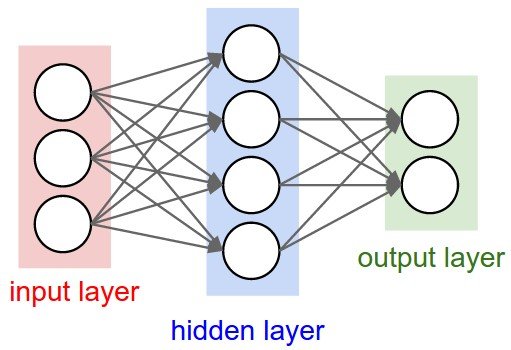
\includegraphics[width=0.6\linewidth]{img/nn/neural_net.jpeg}
  \caption{An sample neural network architecture} 
  \label{fig:sample_nn}
\end{figure}


\chapter{Dependency parsing}
\section{Universal Depndencies}
UD v1.3

\chapter{Neural dependency parser}
\todotext{Tutaj dodać tekst mówiący o czym będzie ten rozdział}
\section{Overview of the network architecture}
The network architecture consists of three main parts: reader, tagger and parser
(see Figure~\ref{fig:architecture}). The reader subnetwork is evaluated on
each individual word in a sentence, and using convolutions on their orthographic
representation produces words embeddings. Next, the tagger subnetwork implemented
as bidirectional RNN equips each word with a context of whole sentence. Finally
parser part computes dependency tree parent for each word using attention mechanism
\cite{vinyals_pointer_2015} after which network computes appropriate dependency label.
In the following paragraphs we will describe all parts in detail.

\begin{figure}[!htbp]
  \centering
  \resizebox{0.8\textwidth}{!}{
    \import{img/network/}{drawing.pdf_tex}
  }
  \caption{The model architecture.} 
  \label{fig:architecture}
\end{figure}

\subsection{Reader}
As stated before the reader subnetwork is run on each word producing its embedding.
This architecture is based on~\cite{kim_character-aware_2015}. Each word $w$
is represented by sequence of its characters plus a special beginning-of-word and
end-of-word tokens. Firstly we find low-dimensional characters embeddings which
are concatenated to form a matrix $C^w$. Then we run 1D convolutional filters
on $C^w$ which then is reduced to vector of filter responses computed as:
\begin{equation} \label{eq:filter_responses}
    R^w_i = \max( C^w \ast F^i )
\end{equation}
Where $F^i$ is i-th filter. The purpose of the convolutions is to react to
specific part of words (because we have bow and eow tokens it can also react to
prefixes and suffixes) which in morphologically rich languages such as Polish   % https://forum.wordreference.com/threads/the-english-language-capital-letter-or-not.2110557/
can depict its grammatical role.

Finally we transform filter responses $R^w$ with a simple multi-layer perceptron
\footnote{Which are just linear transformations followed be non-linearity}
obtaining the final word embedding $E^w = \text{MLP}(R^w)$.

\subsection{Tagger}
Having obtained the word embeddings $E^w$ we can proceed with actually "reading"
whole sentence. To do this we use multi-layer bidirectional RNN (\cite{schuster_bidirectional_1997})
(we have evaluated LSTM~\cite{RNN_LSTM} and GRU~\cite{RNN_GRU} types). We combine
the backward and forward passes by adding them.

\subsubsection{POS tag predictor}
To prevent overfitting and encourage network to compute morphological features
we can add additional training objective. It works by taking output from one of
the tagger BiRNN layers and use it to predict available part-of-speech tags for
each word. The result is not feeded back to the rest of the network because we
think it would introduce too much noise.

\subsection{Parser}
The last part of the network serves two purposes: to find head for each word and
to compute label for that edge.

\subsubsection{Finding head word}
We use method similar to~\cite{vinyals_pointer_2015}.
The input to this part are word annotations $H_0, H_1, \dots, H_n$ (where $H_0$
serves as a root word) produced by the tagger. For each of the words $1,2,\dots,n$
we compute probability distribution which tell us where the head of current
word should be ($0,1,2,\dots,n$). This computation (called \emph{scorer}) is implemented
as small feedforward network $s(w,l) = f(H_w, H_l)$, where $w \in {1,2,\dots,n}$,
$l \in {0,1,2,\dots,n}$.

\subsubsection{Finding edge label}
Output of the scorer can already be interpreted as
pointer network, but in order to use it as attention for computing dependency label
we have to normalize it:
\begin{equation} \label{eq:label_attention}
    p(w,l) = \sum_{i=0}^{n} \frac{f(H_w, H_l)}{f(H_w, H_i)}
\end{equation}
The dependency label is computed by small Maxout network~\cite{goodfellow_maxout_2013},
which takes the current word annotation $H_w$ and heads annotation $A_w$. This
part is called \emph{labeller}.
We investigated two variations of head annotation $A_w$
\\
\\
\\
\emph{Soft attention}\\
Which is a weighted average of normalized attention~\ref{eq:label_attention}
and words annotations $H$. 
$$ A_w = \sum_{i=0}^{n} p(w,i)H_i $$
\\
\emph{Hard attention}\\
Here we use a only head annotation.
$$ A_w = H_h $$
During training we use ground-truth head location, whereas during evaluation
we use head word computed in previous step.

\subsubsection{Decoding algorithm}
The \emph{scorer} give us a $n$x$n+1$ matrix of head dependency preference
for each word. From this matrix we have find a set of dependencies that satisfy
some constraints (exactly one root dependant, no cycles).
We investigated two possibilities for such decoding: a greedy algorithm, and
Chu-Liu-Edmonds~\cite{edmonds_optimim_1966}.

\section{Training}
\subsection{Training criterion}
Every neural network needs a training criterion which will be optimized.
Here we have 3 individual training criterion combined together as linear
combination. Those are:
\begin{itemize}
        \item The negative log-likelihood loss $L_h$ on finding proper head for each
            word. The training signal is propagated from scorer down to the reader.
        \item The negative log-likelihood loss $L_l$ on finding dependency label.
            With soft attention it is propagated through the whole network (excluding
            pos tagging part), while with the hard attention we do not propagate
            through the scorer.
        \item The (optional) negative log-likelihood loss $L_t$ on predicting pos tags.
            This error is backpropagated only through pos-predictor and part of tagger
            down to the reader.
\end{itemize}
So the final loss is:
\begin{equation}\label{eq:neural_loss}
    L = \alpha_hL_h + \alpha_lL_l + \alpha_tL_t
\end{equation}

\subsection{Regularization, optimizer and hyperparameters} \label{sec:basic_params}
Regularization is a essential part of  neural network training. It improves 
generalization and prevents overfitting. One of the most popular regularization
technique is called Dropout~\cite{srivastava_dropout:_2014}. Using it, we randomly
drop part of the connections from a certain network layer during training.
In our case dropout is applied to the \emph{reader} output, between the BiRNN
layers of the \emph{tagger} and to the \emph{labeller}.

The models are trained using Adedelta~\cite{zeiler_adadelta:_2012} learning rule,
with weight decay and adaptive gradient clipping~\cite{chorowski_end--end_2014}.
All experiments are early stopped on validation set UAS.

Hyperparameter selection is crucial for neural networks to obtain good results.
For example, comparing our first experiments with architecture depicted above to
the best single-language results (using the same basic architecture) gave us
about 5\% boost in UAS score on Polish language.

To find the best hyperparameters we have used the Spearmint system~\cite{snoek_practical_2012}
invoked on polish dataset. The chosen parameters are as follows.
The \emph{reader} embeds each character into 15 dimensions, and
contains 1050 filters (50$\cdot$k filters of length k for k = 1, 2,\dots, 6) 
whose outputs are projected into 512 dimensions transformed by a 3 equally
sized layers of feedforward neural network with ReLU activation.
The \emph{tagger} contains 2 BiRNN layers of GRU units with 548 hidden
states for both forward and backward passes which are later aggregated using
addition. Therefore the hidden states of the tagger are also 548-dimensional.
The \emph{POS tag predictor} consists of a single affine transformation
followed by a SoftMax predictor for each POS category.
The \emph{scorer} uses a single layer of 384 tanh for head word
scoring while the \emph{labeller} uses 256 Maxout units
(each using 2 pieces) to classify the relation label
\cite{goodfellow_maxout_2013}. The training cost used the constants
$\alpha_h=0.6, \alpha_l=0.4, \alpha_t=1.0$.
We apply 20\% dropout to the \emph{reader} output, 70\% between the BiRNN
layers of the \emph{tagger} and 50\% to the \emph{labeller}. The weight
decay is 0.95. %Adadelta epsilon annealed from 1e-8 to 1e-12

\section{Multilingual training} \label{sec:neural_multilingual}
The big problem of learning to parse is small number of gold standard dependency
trees for many languages (including Polish). With small number of examples
neural networks do not generalize well and can more easily overfit.
There also exist languages with good, standardized treebank like Czech Prague
Treebank~\cite{prague_treebank}.

Because our model is purely neural network we can incorporate a multitask learning
\cite{caruana_multitask_learning}. It allows the network to learn multiple tasks
at the same time, sharing common patterns and distinguishing differences.
Additionally, because we are using Universal Dependencies treebanks~\cite{nivre_universal_2015}
we have common standardized format across many languages, which allowed for
easy implementation of multitask learning and experiments across different languages.

The multilingual model for $n$ languages can be viewed as $n$ copies of our
basic model, but sharing part of the parameters. To unify input/output for each
of the models we sum possible outputs for each data category (characters,
POS categories, dependency labels). If some category doesn't exist within
a particular language then we use a special UNK token. 
To actually make use of multitask learning we must share at least part of the
parameters of all models. We experimented with different sharing strategies
, from share-everything to only sharing the  \textit{parser} part. Additionally
to prevent over-representation of some
languages during training we sample (on each epoch) only portion of the available
data so that each language have equal number of examples (equal to number of samples
of the smallest language).

\chapter{Results}

\section{Single language}
All experiments depicted in this section are based on a configuration shown in section
~\ref{sec:basic_params}. In Table~\ref{tab:universal} we show our baseline results
for a subset of the UD languages (due to limited computational resources we were
not able to train models for all of them). The results are compared to
SyntaxNet~\cite{andor_globally_2016} and ParseySaurus~\cite{alberti_parsey_saurus_2017},
both from Google. The ParseySaurus is based on SyntaxNet, and uses characters
as input, while the original SyntaxNet uses word embeddings. Both are transition-based,
and need no external POS tagger.
It is worth noting that SyntaxNet has different hyperparameter configuration
for each language, while our parser uses the same configuration across all languages.

\begin{table}[!htbp]
  \centering
  \begin{tabular}{l l | l l | l l | l l}
    language & \#sentences & \multicolumn{2}{c|}{Ours} & \multicolumn{2}{c|}{SyntaxNet} & \multicolumn{2}{c}{ParseySaurus} \\ \hline
    & & UAS & LAS & UAS & LAS & UAS & LAS\\ \hline
    Czech & 87 913 & \textbf{91.41} & \textbf{88.18} & 89.47 & 85.93 & 89.09 & 84.99 \\
    Polish & 8 227 & 90.26 & 85.32 & 88.30 & 82.71 & \textbf{91.86} & \textbf{87.49}\\
    Russian & 5 030 & 83.29 & 79.22 & 81.75 & 77.71 & \textbf{84.27} & \textbf{80.65} \\
    German & 15 892 & 82.67 & 76.51 & 79.73 & 74.07 & \textbf{84.12} & \textbf{79.05}\\
    English & 16 622 & 87.44 & 83.94 & 84.79 & 80.38 & \textbf{87.86} & \textbf{84.45}\\ 
    French & 16 448 & \textbf{87.25} & \textbf{83.50} & 84.68 & 81.05 & 86.61 & 83.1\\
    Ancient Greek & 25 251 & \textbf{78.96} & \textbf{72.36} & 68.98 & 62.07 & 73.85 & 68.1
  \end{tabular}
  \caption{Baseline results of models trained on single languages from
    UD v1.3. Our models use only the orthographic representation of
    tokenized words during inference and works without a separate POS tagger.}
  \label{tab:universal}
\end{table}

In the following sections we will show impact of different network parameters
on the result.

\subsection{Impact of \emph{reader} and \emph{predictor}}
We first inspect the impact of different \emph{reader} and \emph{predictor}
settings.
\begin{table}[!htbp]
  \centering
  \label{tab:results}
  \begin{tabular}{l|cc|cc|cc|}
    training inputs & \multicolumn{2}{c|}{Czech} & \multicolumn{2}{c|}{English} & \multicolumn{2}{c|}{Polish} \\
    & UAS & LAS & UAS & LAS & UAS & LAS \\ 
    \multicolumn{7}{c}{Gold POS tags} \\  \hline
    base word & 
    \textbf{91.7} & \textbf{88} & 
    \textbf{88.6} & 85.1 & 
    \textbf{93.4} & \textbf{89.3} \\
    \multicolumn{7}{c}{Predicted POS tags or no POS tags} \\ \hline
    words & 
    82.4 & 72.1 &
    81.9 & 74.7 & 
    74.6 & 61.6  \\
    chars, soft att. & 
    \textbf{90.1} & 85.7 & % results/inprogress/lab110-01/dependency_norec_smaller_cz/pretraining_best.zip
    86.5 & 82.1 & % results/inprogress/sonata2/dep_en/pretraining_best.zip
    89.1 & 82.5 \\ %results/inprogress/lab110-11/dep_pl_lessclip/pretraining_best.zip
    chars, tags, soft att. & 
    89.6 & 82.8 & % lab110-02 results/inprogress/lab110-02/dependency_norec_smaller_cz_tags/pretraining_best.zip
    86.2 & 81.3 & % results/inprogress/sonata1/dep_en_tags/pretraining_best.zip
    90.4 & 83.9 \\ % results/inprogress/lab110-03/dep_cpw_opt_no_r_tags/pretraining_best.zip
    chars, tags, hard att. & 
    \textbf{90.1} & \textbf{86.7} & % results/inprogress/lab110-01/dependency_norec_smaller_cz_tags_l0_hard_restart/pretraining_best.zip
    \textbf{87.6} & \textbf{83.6} & % sonata2 local_storage/dependency_norec_spbest_en_tags_l0_hard/pretraining_best.zip
    \textbf{91.3} & \textbf{86} \\ % results/inprogress/lab110-17/dependency_norec_smaller_pl_tags_l0_hard/pretraining_best.zip
  \end{tabular}
  \caption{Model performance on selected languages and different training inputs. Experiments were run on \textbf{UD v 1.2}} 
\end{table}

In the upper part "Gold POS tags" we show a favorable situation when we have access
to gold pos tag (approved by a human). The inputs are base words embedded in a vector 
(we replace the \emph{reader} subnetwork with simple, learnable table lookup).
This setting allowed us to obtain best results (especially for Polish) but
gold pos tag are not available in a real-word setting so this result is noted just
as a upper band of the model perfromance.

The "words" and "chars, soft att." settings don't use a \emph{predictor}. Using just words
as inputs (embedded in the same manner as base word) gives worst results. This is
easy to predict because most words in the dataset occurs only once and so the
network doesn't have a clue about role of most of the words.
Instead, using character-level input allows us to obtain much better results, especially
because in morphosyntactically rich languages the word spelling catches many
word features that can be used in deducing the pos tag information.

The result of adding a \emph{predictor} depends on the attention type used.
Used with soft attention it decreased the results in Czech and English, but increased
in Polish. When hard attention is used it can obtain the best results in all cases.
The intuition behind these results is that with hard attention the labeller only
sees annotation of the chosen head, and the error is backpropagated only to this
element. On the other hand with soft attention the head annotation refers
to many incorrect words introducing more noise. Additionally the soft attention labeller
error is backpropagated through all words, which can introduce even more noise on the neural weights.


\subsection{Impact of decoding algorithm}

In the Table~\ref{tab:edmonts_baseline} we show the comparison of greedy and
Chu-Liu-Edmonds decoding algorithms.

\begin{table}[!htbp]
  \centering
  \begin{tabular}{l | c c}
    language & Greedy UAS & Edmonds UAS \\ \hline
      Czech & \textbf{91.41} & 91.40 \\
      Polish &  \textbf{90.26} & 90.17 \\
      Russian & \textbf{83.29} & 83.23 \\
      German &  \textbf{82.67} & 82.66 \\
      English & \textbf{87.44} & 87.41 \\
      French &  \textbf{87.25} & 87.18 \\
      Ancient Greek & \textbf{78.96} & 78.92
  \end{tabular}
  \caption{The comparison of greedy and edmonts decoding algorithms}
  \label{tab:edmonts_baseline}
\end{table}

\begin{figure}[!htbp]
  \centering
  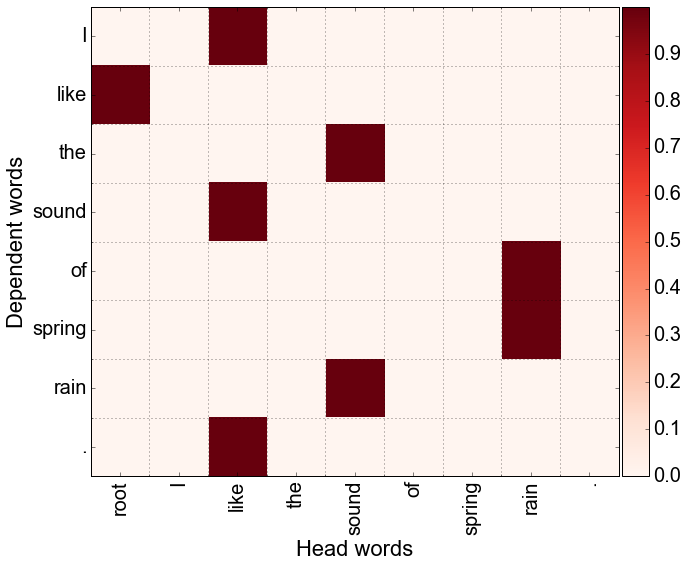
\includegraphics[width=0.6\linewidth]{img/examples/cle/attention.png}
  \caption{A typical scorer output showing probabilities assigned for head-word location.} 
  \label{fig:attention}
\end{figure}

Counter intuitively the CLE algorithm makes the decoding results slightly worse.
We have investigated this and the problem lies in the confidence of the
\emph{scorer} predictions which are very sharp (see Figure~\ref{fig:attention}).
Additionally non-top scores are very noisy and do not reflect  meaningful alternatives,
thus CLE algorithm finds a cycle it is very probable that it will break it
in wrong place, creating another error. The example of such behaviour is depicted
in Figure~\ref{fig:cle}.

\begin{figure}[!htbp]
  \centering
  \resizebox{\textwidth}{!}{
    \import{img/examples/cle/}{cle.pdf_tex}
  }
  \caption{Dependency tree for sentence "What to do to advert the threat lurking on ice?".
    The dashed-dotted (zagrożenia\txtrightarrow lodzie), dotted (czyhającego\txtrightarrow uniknąć)
    and dashed (zagrożenia\txtrightarrow uniknąć) arcs denote, respectively greedy, CLE, and groundtruth decodings.
    The greedy decoder produced the incorrect dependency zagrożenia\txtrightarrow lodzie instead of
    zagrożenia\txtrightarrow uniknąć which created a cycle zagrożenia\txtrightarrow lodzie\txtrightarrow czychającego\txtrightarrow zagrożenia.
    However, the CLE algorithm replaced the good connection
    czyhającego\txtrightarrow zagrożenia with czyhającego\txtrightarrow uniknąć
    which removed the cycle but introduced a new error.} 
  \label{fig:cle}
\end{figure}

We tried to counteract this by using label-smoothing regularization (LSR)
\cite{szegedy_rethinking_2015}.
It is a very simple method of regularization which changes 1-hot vector encoding
of groundtruth data to some other distribution which have effect of lowering overconfidence
of the network. In our case we soften the head position groundtruth vector by
giving the proper head 51\% probability and uniformly distribute the rest 49\%
among other words. Unfortunately this method did not improve the overall CLE algorithm
score.

\subsection{Recurrent state size}
We have also investigated the impact of the \emph{tagger} recurrent state size.
It is desirable to have as small recurrent state size as possible because this
part of the network is activated as many times as there are words in the sentence,
making it a big performance factor.

\begin{table}[!htbp]
    \centering
    \begin{tabular}{l c c c c}
        Language & \% of recurrent state size & UAS & LAS \\ \hline
        \multirow{3}{*}{Polish}& 100\% & 90.26 & 85.32 \\
        & 50\% & \textbf{90.54} & \textbf{85.64} \\
        & 25\% & 89.07 & 82.80 \\ \hline
        \multirow{3}{*}{Czech}& 100\% & \textbf{91.41} & \textbf{88.18}\\
        & 50\% & 89.98 & 85.92\\
        & 25\% & 85.56 & 79.16\\ \hline% ale tutaj to malo epok bylo
    \end{tabular}
    \label{tab:birnn_single_size}
    \caption{Impact of the \emph{tagger} recurrent state size on the performance.
    We report this value as percent of baseline rnn size.}
\end{table}

We can see that in small dataset language like Polish there is not a big difference
between base and 50\% base, whereas in Czech the performance drop is significant.
Because we want to use the same architecture for every language the original 548
units recurrent state size is optimal.

\subsection{Word pieces model}
Following \cite{sennrich_subword_2015} we experimented with subword units.
Instead of using single characters as inputs we can find frequent common characters groups and
depict each word as combination of those units. Of course to be able to
present every word, each single letter also has to be treated as small subword unit. 
For example lets consider two polish words: \emph{lepszy} and \emph{najlepszy} (better, the best).
The \emph{naj} prefix in polish used with adjective means that it is in superlative degree,
so we can imagine that this letter composition is pretty common and thus will be
treated as subword unit. Then those two words will be shown to the network as
\emph{naj-l-e-p-s-z-y} and \emph{l-e-p-s-z-y} (- acting as subword delimiter).

Our word pieces model are obtained as follows:
first we compute word frequency dictionary  and initialize pieces dictionary with all characters in the dataset.
From frequency dictionary we take the most common character bigram and we treat it as new character and replace all previous occurrences
with this new unit. The number of such iterations is a parameter given by the user.
To convert word to pieces we use a greedy strategy. For word $w$ we find the longest
piece $p$ that is prefix of $w$. The next step takes $w$ suffix of size $\|w\| - \|p\|$.

\begin{table}[!htbp]
    \floatbox[{\capbeside\thisfloatsetup{capbesideposition={right,center},capbesidewidth=7cm}}]{figure}[\FBwidth]
    {\caption{Results on word pieces model. \#pieces denotes how many new
    multi-character tokens were used. To convert word to pieces we
    use a greedy algorithm in which we choose the longest piece that is equal
    to prefix of word.}
    \label{tab:word_pieces}}
{
    \begin{tabular}{c c c}
        \#pieces & UAS & LAS \\ \hline
        \multicolumn{3}{c}{Polish}\\
        25 & 90.29 &  84.91 \\
        50 & \textbf{90.40} &  \textbf{85.46}\\
        75 &  90.23 & 84.87\\
        100 & 89.97 & 84.44\\\hline
        \multicolumn{3}{c}{Czech}\\
        25 & 90.29 & 86.50\\
        50 & 90.03 & 86.08\\
        75 & 90.17 & 86.40\\
        100 & \textbf{90.84} & \textbf{87.31}
    \end{tabular}
}
\end{table}

In Table~\ref{tab:word_pieces} we have depicted the results of word pieces model
for different number od additional multi-character tokens. There is only minor
improvement for Polish while for Czech we have actually worse results. Additionally
this input model is not well suited for multilanguage parser, because the pieces
frequency is different for each language.

\section{Multilanguage training}
The main difference between multilanguage and single language configurations is
that we have to decide which parts of the network should have shared weights.
We tested it on 3 language pairs: Polish-Czech, Russian-Czech, Polish-Russian.
They all are from the same Slavic family, but Russian uses Cyrillic alphabet as
opposed to Latin script for Polish and Czech. The main advantage of Czech language
that made us choose it as auxiliary language is the quality and quantity of training data
- it is over 6 times bigger than Polish and Russian datasets combined.
The results of different sharing strategies are depicted in Table~\ref{tab:multi_baseline}.

\begin{table}[!htbp]
  \centering  
  \begin{tabular}{l | l l c c}
    Shared parts & Main lang & Aux lang & UAS & LAS \\ \hline
      - & Polish & - & 90.31 & 85.21 \\
    \emph{Parser} & Polish & Czech & 90.72 & 85.57 \\ % local_storage/multi/pl_cs_merge_generator
    \emph{Tagger, Parser} & Polish & Czech & 91.19 & 86.37 \\ % sonata2:  /pio/lscratch/1/i248100/pl_cs_unification_exclude_pos
    \emph{Tagger, POS Predictor, Parser} & Polish & Czech & 91.65 & 86.88 \\ % local_storage/dependency_pl_cs_new
    \emph{Reader, Tagger, POS Predictor, Parser} & Polish & Czech & \textbf{91.91} & \textbf{87.77} \\\hline % sonata1: /pio/lscratch/1/i248100/multi_pl_cs_different_eos_merge_all
    \emph{Parser} & Polish & Russian & 90.31 & 85.07 \\  % local_storage2/pl-ru-inc-generator
    \emph{Tagger, POS Predictor, Parser} & Polish & Russian &
    \textbf{91.34} & \textbf{86.36} \\ 
    \emph{Reader, Tagger, POS Predictor, Parser} & Polish & Russian & 89.16 & 82.94 \\  %  local_storage2/multi_pl_ru_different_eos_merge_all
\hline\hline % local_storage/multi/pl_ru_same_eos
    - & Russian & - & 83.43 & 79.24 \\
    \emph{Parser} & Russian & Czech & 83.15 & 78.69 \\  % sonata0: /pio/lscratch/1/i248100/ru-cs-parser
    \emph{Tagger, POS Predictor, Parser} & Russian & Czech & 83.91 & 79.79 \\ %  local_storage/multi/ru_cs
    \emph{Reader, Tagger, POS Predictor, Parser} & Russian & Czech & \textbf{84.78} & \textbf{80.35} % sonata1:  /pio/lscratch/1/i248100/ru-cs-all
  \end{tabular}
  \label{tab:multi_baseline}
  \caption{Impact of parameter sharing strategies on main language parsing accuracy when multilingual training
    is used for additional supervision.}
\end{table}


Multilingual training (Table~\ref{tab:multi_baseline}) improves the performance on low-resource languages.
We observe that the optimal amount of parameter sharing depends on the similarity
between languages and corpus size – while it is beneficial to share all parameters of the
PL-CZ and RU-CZ parser, the PL-RU parser works best if the reader subnetworks are
separated. 

Similarly as in the single language configuration we have tested the impact of \emph{tagger}
recurrent state size on the results (see Table~\ref{tab:birnn_multi_size}).

\begin{table}[!htbp]
    \centering
    \begin{tabular}{l c c c}
        \% of recurrent state size & UAS & LAS \\ \hline 
        200\% & 91.45 & 86.36\\
        100\% & \textbf{91.65} & \textbf{86.88}\\
        50\% & 89.53 & 83.66\\
        25\% & 87.28 & 78.93
    \end{tabular}
    \label{tab:birnn_multi_size}
    \caption{Impact of the \emph{tagger} recurrent state size on the performance
    of multilanguage pl-cz model.
    We report this value as percent of baseline rnn size.}
\end{table}

The results are computed on best Polish-Czech model (with share all strategy). We can see
that the recurrent state size have similar behaviour as in the single language Czech model - 
the 50\% size has significant drop in the performance. It is worth noting that
increasing the size changes the result only slightly (and that they are actually worse).
This mean that chosen \emph{tagger} size is well-suited for both single and multi
language parsers.

\subsection{Polish-Polish multilang parser}
After investigating results of the parser (this problem applies to both single
and multi parser) we have found that if the \emph{tagger} assigns wrong POS tag to
a particular word it can mislead the scorer and labeller producing wrong parse tree.
In many cases after replacing wrong word with its synonym such that the \emph{tagger}
will assign the right POS tag - the tree becomes a valid parse. For an example see Figure~\ref{fig:pos_bad_good}.

\begin{figure}[htbp]
  \centering
  \resizebox{0.8\textwidth}{!}{
    {\Large
      \import{img/examples/pos/}{bogumil.pdf_tex}
    }
  }
  \\[5pt]
  \resizebox{0.8\textwidth}{!}{
    {\Large
      \import{img/examples/pos/}{michal.pdf_tex}
    }
  }
  \caption{In the upper panel the sentence "Bogumił felt silent so
    much that he almost stopped breathing." is incorrectly parsed.
    We attribute the error to the \emph{reader} or to the \emph{tagger} because the predicted POS
    tag for "Bogumił", a male given name, is wrong (VERB instead of
    NOUN). In the lower panel we replace "Bogumił" with the  more common "Michał" the network assigns
    a proper tag and the whole sentence becomes a valid parse tree.} 
  \label{fig:pos_bad_good}
\end{figure}

The prevent this behaviour on Polish language we have decided to use additional data
for training the \emph{predictor} subnetwork. We used the \emph{milionowy podkorpus} (milion subcorpus)
of the National Corpus of Polish Language \cite{przepiorkowski_nkjp_2012}. We converted
this data to UD conllu format by filling the dependency information with a blank values
and transoforming the polish-style POS tags to UD-style using conversion table provided
by UD authors.
Next we used our multilingual training procedure in which the first langauge was
a standard UD Polish dataset, and the second one was our converted polish subcorpus.
The difference with previous attempts is that we have to ignore loss on dependency head
$L_h$ and dependency label $L_l$ for the second language.\\
This model allowed us to obtain our best results: \textbf{92.69\% UAS} and \textbf{88.92\% LAS}.

\chapter{Summary}
We have demonstrated a graph-based dependency parser implemented as a single deep
neural network that directly produces parse trees from characters and does not require
other NLP tools such as a POS tagger. The parser is trained in an end-to-end manner,
and has separate cost terms that pertain to label accuracy,
head word localization and optionally POS tagging. On
morphologically rich languages the parser is competitive
with other state-of-the-art parsers.
We have established that the multilingual training performance depends heavily
on degree of parameter sharing, and can differ depending on language similarity
and corpus size.


%%%%% BIBLIOGRAFIA

%\bibliographystyle{plain}
\bibliographystyle{apalike}
\bibliography{thesis}

%\begin{thebibliography}{1}
%\bibitem{example} \ldots
%\end{thebibliography}

\end{document}
